\documentclass[pdflatex,sn-mathphys-num]{sn-jnl}% Springer Nature LaTeX template

\usepackage{amsmath,amssymb}
\usepackage{graphicx}
\usepackage{adjustbox}
\usepackage{booktabs}
% Typographic improvements and better line breaking
\usepackage[protrusion=true,expansion=true]{microtype}
\usepackage{xurl} % allow line breaks in long URLs/DOIs
\Urlmuskip=0mu plus 1mu
% Diagram
\usepackage{tikz}
\usetikzlibrary{arrows.meta,positioning,shapes.geometric}
% Keep floats (figures/tables) from escaping their sections
\usepackage{placeins}
\raggedbottom
% Mitigate overfull/underfull boxes in tight paragraphs
\setlength{\emergencystretch}{3em}

% Avoid hyperref bookmark warnings from \paragraph headings
\AtBeginDocument{\hypersetup{bookmarksdepth=3}}

\begin{document}

\title[Three-Stage Bearing Health Classification]{Three-Stage Bearing Health Classification Using Vibration Short-Time Fourier Transform and Temperature Trends in a Run-to-Failure Setting}

\author[1]{\fnm{Long} \sur{Truong}}\email{longt5@fpt.edu.vn}
\equalcont{These authors contributed equally to this work.}

\author*[2]{\fnm{Phu~Le} \sur{Nguyen}}\email{lpnguyen@ntt.edu.vn}
\equalcont{These authors contributed equally to this work.}

\affil[1]{\orgname{Faculty of Engineering and Technology, FPT University}, \orgaddress{\city{Ho Chi Minh City}, \country{Vietnam}}}
\affil[2]{\orgname{Faculty of Engineering and Technology, Nguyen Tat Thanh University}, \orgaddress{\city{Ho Chi Minh City}, \country{Vietnam}}}

\abstract{In this work, the three-stage bearing health classification (Healthy, Degrading, Fault) under a run-to-failure setting is addressed using vibration short-time Fourier transform (STFT) representations and compact temperature trend descriptors. A lightweight multi-modal pipeline is presented in which per-frequency (across-time) normalization stabilizes spectrogram brightness and a late head fuses a minimal 6-D temperature descriptor with vibration features. Evaluation is conducted with a leakage-aware, time-to-failure\,\mbox{(TTF)}-aligned protocol and a two-phase workflow (stratified pre-training followed by temporal fine-tuning) to mitigate temporal leakage and reflect deployment. On a stratified development split, Macro-F1 is $\approx$ 0.7762. Under leakage-aware temporal testing, strong late-life discrimination is achieved (Fault F1 $=0.9600$ on 90--100.1\% TTF), and full-lifecycle performance reaches Accuracy $=0.8915$ and Macro-F1 $=0.8739$ with majority vote, demonstrating clear gains over a vibration-only baseline.}

\keywords{bearing health monitoring, run-to-failure, degradation stage classification, STFT spectrogram, vibration--temperature fusion, temporal split, condition-based maintenance}

\maketitle
\section{Introduction}
\label{sec:intro}

This work targets two practical challenges in run-to-failure bearing monitoring: (i) reliable recognition of the \emph{degrading} stage—often subtle and class-imbalanced—and (ii) \emph{leakage-aware} evaluation that reflects deployment reality rather than optimistic window-level splits \cite{jung2024dib_rtf,kaufman2012leakage,bergmeir2012timeseriescv}. A lightweight multi-sensor approach is adopted in which vibration provides time--frequency evidence and temperature contributes complementary trends near degradation onset \cite{baltrusaitis2019multimodal}. STFT-based CNN features are coupled with a compact temperature descriptor via late fusion, and validation is conducted using a contiguous, TTF-aligned protocol.
To bridge development and deployment, a two-phase workflow is followed: file-wise stratified training for model selection, then temporal fine-tuning aligned with the TTF axis (train [0,60]\%, val [60,70]\%, test [70,100.1]\%) to test generalization from earlier to later life while reducing overlapped-window leakage.
\textbf{Contributions.} This paper makes the following contributions, focusing on what is new and practically useful:
\begin{itemize}
    \item A compute-efficient multi-modal pipeline is proposed that fuses STFT-based two-axis vibration features with a minimal 6-D temperature trend/statistical descriptor via a late-fusion head, together with per-frequency (across-time) normalization to stabilize spectrogram brightness.
    \item A leakage-aware, TTF-aligned evaluation recipe with present-class scoring and file-wise mean-logit aggregation is employed to reflect deployment and avoid window-overlap leakage; the protocol makes performance interpretation robust when some classes are absent late in life.
    \item Targeted ablations (vibration-only vs. multi-modal, stratified initialization vs. scratch, temporal slice selection) are provided to explain when temperature adds value and how initialization affects temporal generalization.
    \item Empirically, strong performance is achieved: Macro-F1 $\approx$ 0.7762 on a 3-class stratified split; under leakage-aware temporal testing (present classes), \textbf{Early (70--90\%): Accuracy $=0.8846$, Degrading F1 $=0.9388$} and \textbf{Late (90--100.1\%): Accuracy $=0.9231$, Fault F1 $=0.9600$}. Over the full range $[0,100.1]\%$ with majority vote, Accuracy $=0.8915$ and Macro-F1 $=0.8739$.
\end{itemize}

\section{Related Work}
Time--frequency CNNs have been studied extensively for bearing fault diagnosis and provide strong baselines under controlled settings \cite{zhao2019deep,lei2020roadmap,ince2016tie,wen2018neurocomputing}. Transfer learning further improves robustness and data efficiency across domains \cite{shao2019tii_transfer}. Beyond single-modality vibration, multimodal methods combine complementary signals (e.g., temperature) to enhance robustness near degradation onset \cite{baltrusaitis2019multimodal,huo2022tim_multisensor,gao2024inffus_multisource,xiao2025inffus_multilevel}. However, many prior studies rely on random/window-level splits that can introduce temporal leakage and overly optimistic estimates. In contrast, this work adopts a \emph{leakage-aware, TTF-aligned} evaluation that respects chronology and reports present-class metrics when some classes are absent, providing a more deployment-oriented assessment.

\section{Methodology}
\label{sec:method}

\subsection{Overview}
A lightweight multi-modal pipeline is presented. Each 1.0-s window yields a 2-channel log-spectrogram from two-axis vibration and a compact 6-D descriptor from two-channel temperature. A small 2D CNN encodes vibration, a linear layer embeds temperature, and a late-fusion classifier predicts the stage. Training is two-phase: file-wise stratified learning followed by leakage-aware temporal fine-tuning aligned with the TTF axis. Figure~\ref{fig:block} summarizes the end-to-end flow and where fusion and file-wise aggregation occur.

\begin{figure}[t]
  \centering
  \begin{adjustbox}{max width=\linewidth}
  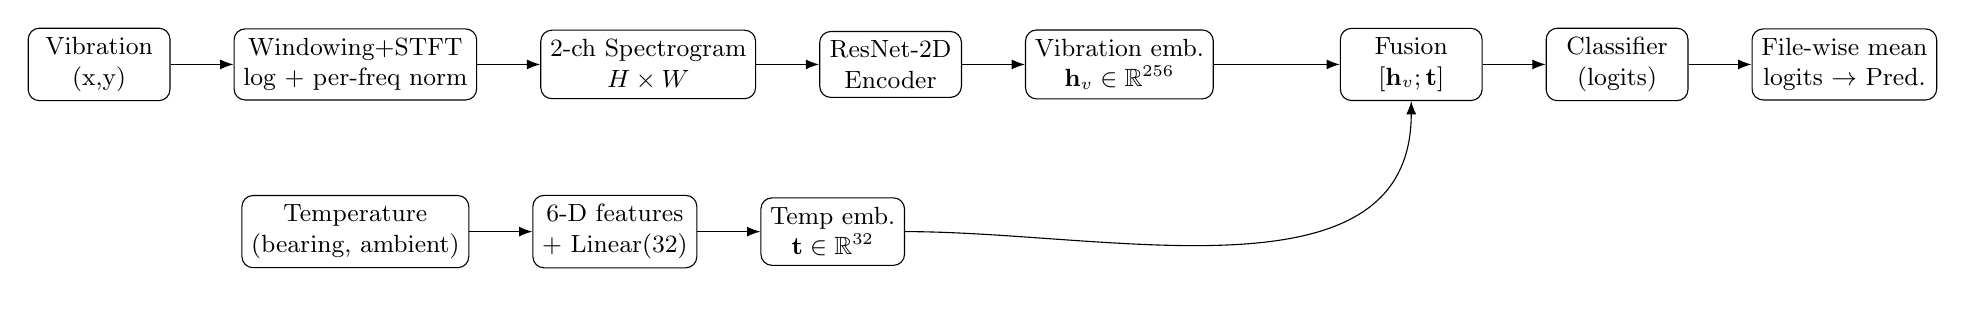
\begin{tikzpicture}[
    node distance=8mm and 8mm,
    box/.style={draw, rounded corners, align=center, minimum height=7mm, minimum width=18mm, font=\small},
    arr/.style={-Latex}
  ]
    % Top chain (compact)
    \node[box] (vib) {Vibration\\(x,y)};
    \node[box, right=of vib] (wstft) {Windowing+STFT\\log + per-freq norm};
    \node[box, right=of wstft] (spec) {2-ch Spectrogram\\$H\times W$};
    \node[box, right=of spec] (cnn) {ResNet-2D\\Encoder};
    \node[box, right=of cnn] (vz) {Vibration emb.\\$\mathbf{h}_v\in\mathbb{R}^{256}$};

    % Temp branch (compact)
    \node[box, below=12mm of wstft, xshift=0mm] (temp) {Temperature\\(bearing, ambient)};
    \node[box, right=of temp] (tfeat) {6-D features\\+ Linear(32)};
    \node[box, right=of tfeat] (tz) {Temp emb.\\$\mathbf{t}\in\mathbb{R}^{32}$};

    % Fusion + classifier + aggregation
    \node[box, right=16mm of vz] (fuse) {Fusion\\$[\mathbf{h}_v;\mathbf{t}]$};
    \node[box, right=of fuse] (cls) {Classifier\\(logits)};
    \node[box, right=of cls] (agg) {File-wise mean\\logits $\to$ Pred.};

    % Arrows top chain
    \draw[arr] (vib) -- (wstft);
    \draw[arr] (wstft) -- (spec);
    \draw[arr] (spec) -- (cnn);
    \draw[arr] (cnn) -- (vz);

    % Temp arrows
    \draw[arr] (temp) -- (tfeat);
    \draw[arr] (tfeat) -- (tz);

    % Fusion arrows
    \draw[arr] (vz) -- (fuse);
    % Route temp embedding to fusion from below to avoid crossing blocks
    \draw[arr] (tz.east) to[out=0,in=270] (fuse.south);
    \draw[arr] (fuse) -- (cls);
    \draw[arr] (cls) -- (agg);
  \end{tikzpicture}
  \end{adjustbox}
  \caption{Block diagram of the proposed multi-modal pipeline with late fusion and file-wise mean-logit aggregation.}
  \label{fig:block}
\end{figure}

\subsection{Signal Processing and Feature Extraction}
Vibration (2 axes) and temperature (2 channels) are sampled synchronously and sliced by identical 1.0-s windows with 50\% overlap, avoiding extra timestamp alignment. (If rates differ in deployment, a simple resampling/alignment step is required.)

Each window is sanitized (NaN/Inf \,\,$\to$\,0) and z-scored per channel. STFT log-magnitude spectrograms are computed with $n\_{fft}=2048$, $hop\_length=512$ (Hann), then resized to $160\times160$. A per-frequency (across-time) normalization stabilizes spectral brightness; the two vibration axes are then stacked as channels to form a $(2\times H\times W)$ input. In parallel, a compact 6-D temperature descriptor (mean, std, slope for each of two channels) is computed per window.

\subsection{Model and Fusion Head}
Standard late fusion: concatenate the vibration embedding with the temperature embedding, then apply a linear head to produce logits.

\subsection{Inference and Metrics}
\label{sec:filewise}\label{sec:present}
For each file, average \emph{pre-softmax} logits across windows (mean-logit) and take $\arg\max$ over the mean. Let $\mathcal{F}$ be the set of files in an evaluation slice and $\mathcal{C}$ the set of stage labels. For file $f\in\mathcal{F}$ with window set $\mathcal{W}_f$, the model produces per-window logits $\mathbf{z}_w\in\mathbb{R}^{|\mathcal{C}|}$. We compute mean-logits and a file-level prediction as
\begin{equation*}
\bar{\mathbf{z}}_f = \frac{1}{|\mathcal{W}_f|}\sum_{w\in\mathcal{W}_f} \mathbf{z}_w,\quad \hat{y}_f = \arg\max_{c\in\mathcal{C}} (\bar{\mathbf{z}}_f)_c.
\end{equation*}
Define the \emph{present-class} set $\mathcal{P} = \{ c\in\mathcal{C} : \text{support}(c) = |\{ f\in\mathcal{F} : y_f = c \}| > 0 \}$. We compute per-class precision/recall/F1 only for $c\in\mathcal{P}$:
\begin{align*}
\mathrm{Prec}_c &= \frac{\mathrm{TP}_c}{\mathrm{TP}_c + \mathrm{FP}_c},\quad
\mathrm{Rec}_c = \frac{\mathrm{TP}_c}{\mathrm{TP}_c + \mathrm{FN}_c},\\
\mathrm{F1}_c &= \frac{2\,\mathrm{Prec}_c\,\mathrm{Rec}_c}{\mathrm{Prec}_c + \mathrm{Rec}_c} \quad (\text{defined when denominator} > 0).
\end{align*}
Macro-F1 over present classes is then
\begin{equation*}
\mathrm{Macro\text{-}F1}_{\text{present}} = \frac{1}{|\mathcal{P}|}\sum_{c\in\mathcal{P}} \mathrm{F1}_c.
\end{equation*}
When an evaluation slice becomes single-class (e.g., very late life), we report the per-class F1 for the present class and omit Macro-F1 (marked as \textemdash{} in tables).

\subsection{Training and Evaluation Protocol}
Training first proceeds under a file-wise stratified split, then fine-tuning uses a leakage-aware temporal split aligned with TTF: train [0,60]\%, val [60,70]\%, test [70,100.1]\%. Hyperparameters and settings for both phases are summarized in Table~\ref{tab:settings}; full experimental details are provided in Section~\ref{sec:exp_setup}.

\section{Experimental Setup}
\label{sec:exp_setup}

\subsection{Experimental Configuration}
The run-to-failure bearing dataset provided by Jung et al.~\cite{jung2024dib_rtf,jung2024mendeley_rtf} is used in this study. 
The dataset contains \textbf{one run} (\texttt{RUNS=1}) consisting of \textbf{129 files} (\texttt{FILES=129}). 
Two-axis vibration signals are sampled at \textbf{25.6 kHz}.

Vibration is segmented into fixed-length windows of \textbf{1.0 s} (25{,}600 samples) with \textbf{50\% overlap} (hop = 0.5 s = 12{,}800 samples). 
Each vibration window is converted to a time--frequency representation using STFT with $n\_fft=2048$ and $hop\_length=512$. 
The resulting spectrogram is resized to \textbf{$160\times160$} for both the development and temporal fine-tuning settings in this work.

In addition, temperature features are extracted from \textbf{two channels}. 
For each window, \textbf{six} temperature descriptors are computed: mean, standard deviation, and slope for each channel (total 6-D).

Let $\mathrm{TTF\%} \in [0,1]$ denote the normalized time-to-failure percentage within the run. 
Three stages are defined along normalized lifetime; see Table~\ref{tab:stages} for the threshold ranges that delineate early/mid/late life and guide temporal splits.
\begin{table}[t]
  \centering
  \caption{Health stages by TTF\% (normalized lifetime).}
  \label{tab:stages}
  \begin{tabular}{lc}
    \toprule
    Stage & TTF\% range \\
    \midrule
    Healthy & $[0,0.60)$ \\
    Degrading & $[0.60,0.90)$ \\
    Fault & $[0.90,1.00]$ \\
    \bottomrule
  \end{tabular}
\end{table}
\noindent\textit{Note:} Evaluation slices sometimes use $100.1\%$ as a technical padding to ensure full coverage of the last file in a run.

All experiments run on a single NVIDIA RTX 2060 (6\,GB) GPU with PyTorch~2.x and CUDA~12.x. Unless stated otherwise, the random seed is fixed to 42 for both data splitting and training. Final results use the configuration at \verb|configs/logs_stft_full_temporal_gating.yaml| and the corresponding checkpoint produced in \verb|runs/logs_stft_temporal_gating_final|. Mixed precision (AMP) is enabled; for temporal evaluation, up to 50 validation windows per file are used (\verb|val_max_windows=50|).

\subsection{Development setting: stratified split}
A file-wise stratified split is adopted for development (0.6/0.2/0.2). Training hyperparameters and settings are summarized in Table~\ref{tab:settings}.

\begin{table}[htbp]
\caption{Training settings (dev vs. temporal fine-tuning).}
\label{tab:settings}
\centering
\begin{tabular}{lcc}
\toprule
 & Stratified (dev) & Temporal (FT) \\
\midrule
Optimizer & AdamW & AdamW \\
LR & $2\times10^{-4}$ & $3\times10^{-5}$ \\
Weight decay & $10^{-3}$ & $10^{-2}$ \\
Epochs & 80 & 60 \\
Schedule & -- & cosine (OneCycle off) \\
\bottomrule
\end{tabular}
\end{table}

\subsection{Deployment-oriented setting: leakage-aware temporal split}
A contiguous, TTF-aligned temporal split is adopted to avoid overlapped-window leakage and better match deployment: train [0,60]\%, val [60,70]\%, test [70,100.1]\%. The split is illustrated in Figure~\ref{fig:protocol_compare}; remaining settings follow Table~\ref{tab:settings}.

\begin{figure}[t]
  \centering
  \begin{minipage}[b]{0.47\textwidth}
    \centering
    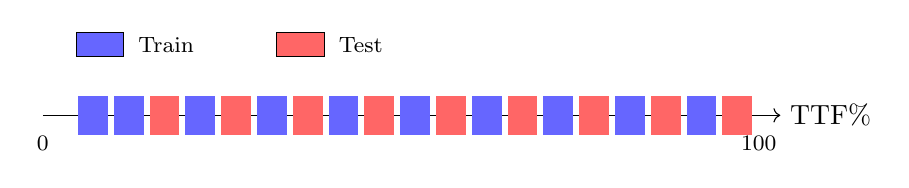
\begin{tikzpicture}[x=0.075\linewidth, y=6mm]
      % Time-to-failure (TTF) axis
      \draw[->] (0,0) -- (10.3,0) node[right]{TTF\%};
      \node at (0,-0.6){\footnotesize 0}; \node at (10,-0.6){\footnotesize 100};
      
      % Alternating window blocks (Train/Test) illustrating leakage risk
      \foreach \x/\c in {0.5/blue!60,1/blue!60,1.5/red!60,2/blue!60,2.5/red!60,3/blue!60,3.5/red!60,4/blue!60,4.5/red!60,5/blue!60,5.5/red!60,6/blue!60,6.5/red!60,7/blue!60,7.5/red!60,8/blue!60,8.5/red!60,9/blue!60,9.5/red!60} {
        \draw[fill=\c,draw=\c] (\x,-0.4) rectangle ++(0.4,0.8);
      }
      
      % Legend (kept minimal to balance subfig heights)
      \draw[fill=white, draw=white] (0.5,1.38) rectangle (3.4,1.62);
      \node[draw, fill=blue!60, minimum width=6mm, minimum height=3mm] (l1) at (0.8,1.5) {};
      \node[anchor=west] at (1.2,1.5) {\footnotesize Train};
      \node[draw, fill=red!60, minimum width=6mm, minimum height=3mm] (l2) at (3.6,1.5) {};
      \node[anchor=west] at (4,1.5) {\footnotesize Test};
    \end{tikzpicture}
  \end{minipage}
  \hfill
  \begin{minipage}[b]{0.47\textwidth}
    \centering
    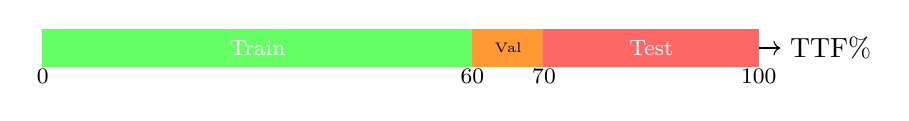
\begin{tikzpicture}[x=0.075\linewidth, y=6mm]
      % Time-to-failure (TTF) axis
      \draw[->] (0,0) -- (10.3,0) node[right]{TTF\%};
      \node at (0,-0.6){\footnotesize 0}; \node at (6,-0.6){\footnotesize 60}; \node at (7,-0.6){\footnotesize 70}; \node at (10,-0.6){\footnotesize 100};
      
      % Contiguous temporal split blocks (Train 60%, Val 10%, Test 30%)
      \draw[fill=green!60,draw=green!60] (0,-0.4) rectangle (6,0.4);
      \node[color=white, font=\footnotesize] at (3,0) {Train};
      \draw[fill=orange!80,draw=orange!80] (6,-0.4) rectangle (7,0.4);
      \node[font=\tiny] at (6.5,0) {Val};
      \draw[fill=red!60,draw=red!60] (7,-0.4) rectangle (10,0.4);
      \node[color=white, font=\footnotesize] at (8.5,0) {Test};
    \end{tikzpicture}
  \end{minipage}
  
  \caption{Protocol comparison. Left: window-level random split (leakage risk). Right: contiguous TTF\-aligned temporal split (leakage-aware).}
  \label{fig:protocol_compare}
\end{figure}

\section{Results}
\label{sec:results}

\subsection{Stratified evaluation (3-class)}
In the stratified development setting, the best configuration (\texttt{auto\_r22}) achieves \textbf{Macro-F1 = 0.7762}. 
Per-class F1 scores are approximately: Healthy $\approx$ 0.69, Degrading $\approx$ 0.64, and Fault = 1.00. 
This indicates that Fault signatures are highly separable, while the Degrading stage remains the most challenging due to its transitional nature.

These stratified results are summarized in text for brevity.

\subsection{Temporal evaluation (deployment-oriented)}
Under the temporal leakage-aware split, the test slice [70,100.1]\% corresponds to late-life behavior where \emph{Healthy samples do not appear}. 
Therefore, metrics are reported over the \emph{present classes} (Degrading and Fault). 
Using mean-logit aggregation on the best temporal configuration, the model attains \textbf{Early (70--90\%): Accuracy = 0.8846 (Degrading only; F1 = 0.9388)} and \textbf{Late (90--100\%): Accuracy = 0.9231; Fault F1 = 0.9600}. 
These results suggest that the learned representation transfers from earlier life to late-life conditions; the Healthy--Degrading boundary around 60--70\% TTF remains the main challenge when broader coverage is included.

Figure~\ref{fig:temporal_pair} summarizes temporal performance on the late-life slice.
\begin{figure}[t]
  \centering
  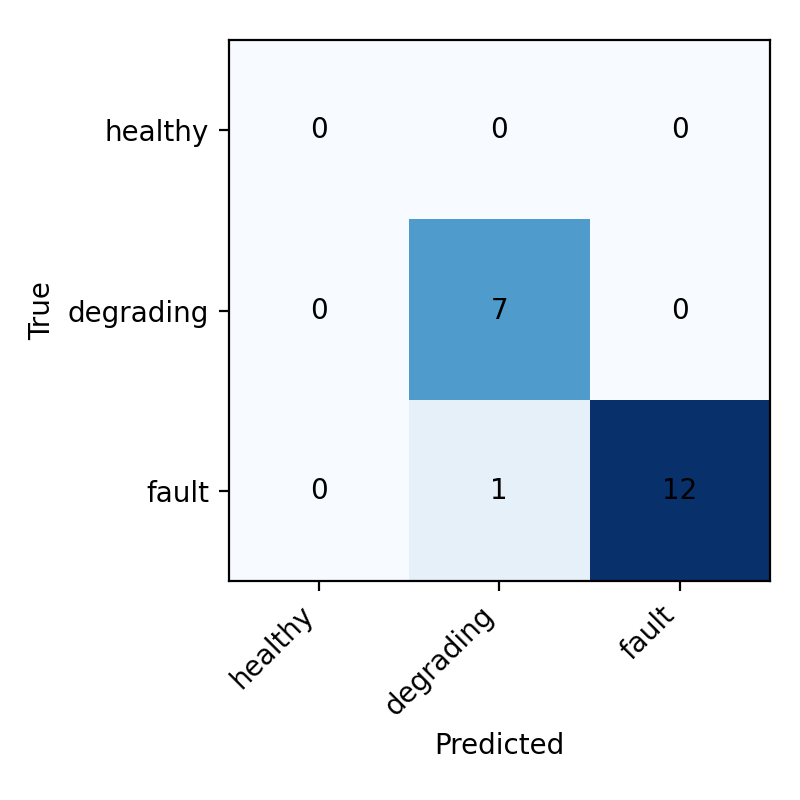
\includegraphics[width=0.48\linewidth]{figures/temporal/confusion_matrix.png}
  \hfill
  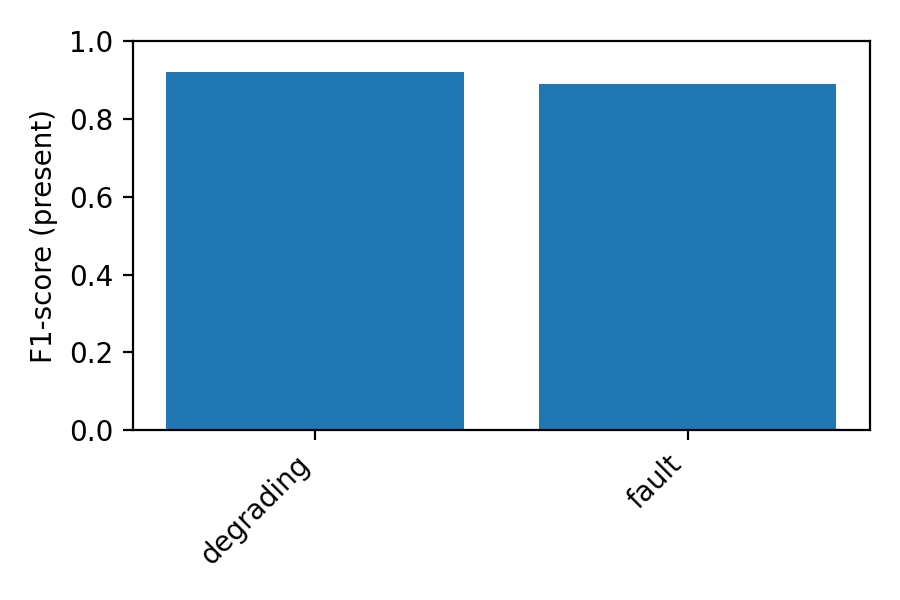
\includegraphics[width=0.48\linewidth]{figures/temporal/f1_present.png}
  \caption{Leakage-aware temporal evaluation on the late-life slice [70,100.1]\% TTF. Left: confusion matrix. Right: per-class F1 over present classes (Healthy absent).}
  \label{fig:temporal_pair}
\end{figure}

\subsection{Full-range temporal (0--100.1\%)}
The final model is further evaluated over the entire lifecycle $[0,100.1]\%$ TTF. With \textbf{majority vote} aggregation, the model attains \textbf{Accuracy $=0.8915$} and \textbf{Macro-F1 $=0.8739$}. Using \textbf{mean-logit} aggregation, Accuracy is $=0.7752$ and Macro-F1 is $=0.8006$. See Figure~\ref{fig:fullrange_pair} for a visual summary.
\begin{figure}[t]
  \centering
  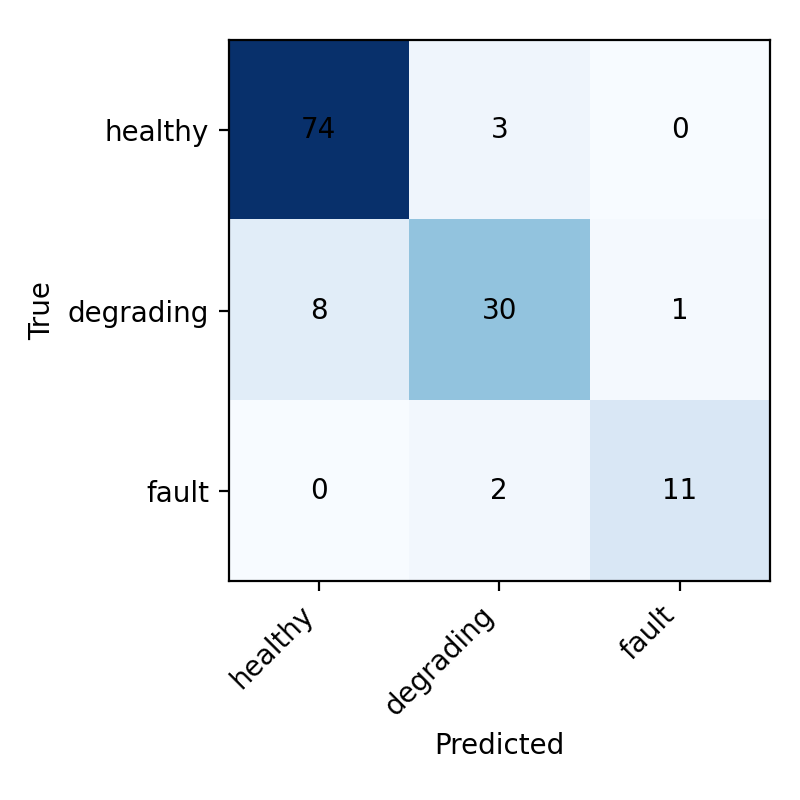
\includegraphics[width=0.48\linewidth]{figures/fullrange/confusion_matrix_full.png}
  \hfill
  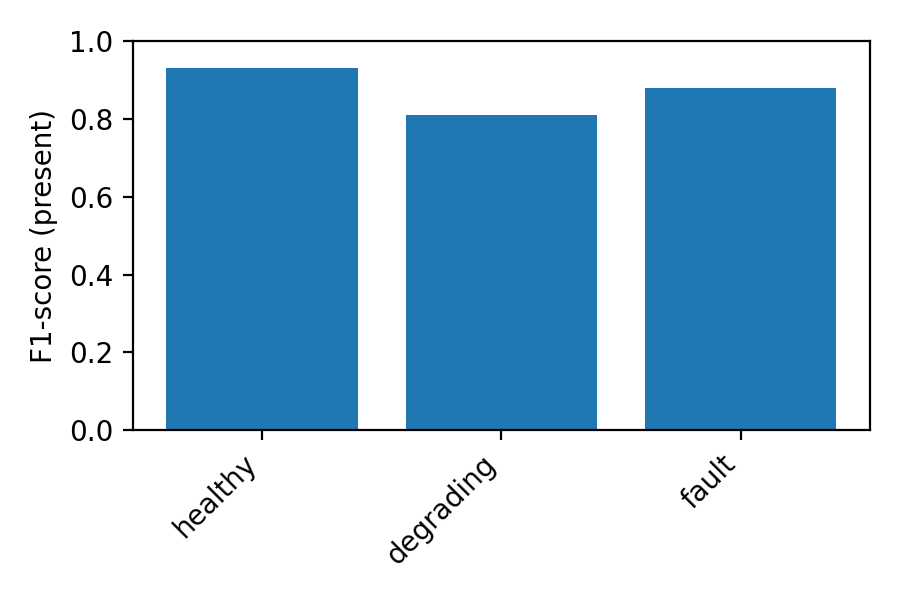
\includegraphics[width=0.48\linewidth]{figures/fullrange/f1_present_full.png}
  \caption{Full-range temporal evaluation $[0,100.1]\%$ TTF (file-wise aggregation). Left: confusion matrix. Right: per-class F1.}
  \label{fig:fullrange_pair}
\end{figure}

\subsection{Failure case analysis with broader temporal coverage}
When evaluation expands to cover a broader range that includes more ambiguous mid-life samples, metrics can shift notably: Degrading is more frequently confused with Healthy and, depending on the slice, Healthy may have zero support. This highlights sensitivity near the Healthy--Degrading boundary and motivates stronger supervision and longer temporal context.

\FloatBarrier
\section{Ablation and Discussion}
\label{sec:discussion}
\subsection{Ablation Studies}
\label{sec:ablation}

Table~\ref{tab:abl_summary} consolidates ablations across temporal slices. In particular, on a representative late-life slice $[85,100.1]\%$, the multi-modal model (vibration+temperature) attains Macro-F1 $=0.9467$ versus $0.2593$ for vibration-only, with Fault F1 improving from $0.0000$ to $0.9600$, underscoring the benefit of multi-sensor fusion near transition and late stages. Key takeaways:
\begin{itemize}
  \item \textbf{Modality effect.} On late-life slices, the vibration-only model fails to detect Fault (F1 $\approx$ 0.00), while the multi-modal model achieves strong Fault recognition (e.g., 0.9600 at $[90,100.1]\%$, 0.8889 at $[70,100.1]\%$).
  \item \textbf{Initialization.} Initializing temporal fine-tuning from the best stratified checkpoint outperforms training from scratch (same coverage).
  \item \textbf{Slice sensitivity.} Broader coverage $[70,100.1]\%$ reduces Degrading F1 due to the Healthy--Degrading boundary; very-late $[90,100.1]\%$ can become single-class (Fault).
  \item \textbf{Classical baseline.} An 8D vib SVM is competitive on $[70,90]\%$ (Degrading-only) but collapses on very-late slices, underscoring the need for the leakage-aware protocol and multi-modal cues.
  \item \textbf{Variants.} Removing class-weights or switching to higher resolution (4096/1024, 224$\times$224) underperforms the final configuration.
\end{itemize}

\begin{table}[t]
  \caption{Consolidated ablation summary across temporal slices (present-label metrics where applicable). \emph{Note:} \textemdash{} indicates metrics not applicable due to absent labels or single-class slices.}
  \label{tab:abl_summary}
  \centering
  \begin{tabular}{l l c c c c}
    \toprule
    Slice & Variant & Accuracy & Macro-F1 (present) & F1 Degrading & F1 Fault \\
    \midrule
    $[70,90]\%$ & Multi-modal (vib+temp) & 0.8846 & \textemdash{} & 0.9388 & \textemdash{} \\
    $[70,90]\%$ & Classical vib (SVM, 8D) & 1.0000 & \textemdash{} & 1.0000 & \textemdash{} \\
    $[85,100.1]\%$ & Vib-only &  & 0.2593 & 0.5185 & 0.0000 \\
    $[85,100.1]\%$ & Multi-modal (vib+temp) &  & 0.9467 & 0.9333 & 0.9600 \\
    \midrule
    $[70,100.1]\%$ & Vib-only &  & 0.8000 & 0.8000 & 0.0000 \\
    $[70,100.1]\%$ & Classical vib (SVM, 8D) & 0.6667 & 0.4000 & 0.8000 & 0.0000 \\
    $[70,100.1]\%$ & Multi-modal (vib+temp) & 0.8974 & 0.9045 & 0.9200 & 0.8889 \\
    \midrule
    $[90,100.1]\%$ & Multi-modal (vib+temp) & 0.9231 & \textemdash{} & \textemdash{} & 0.9600 \\
    $[90,100.1]\%$ & Classical vib (SVM, 8D) & 0.0000 & \textemdash{} & \textemdash{} & 0.0000 \\
    $[90,100.1]\%$ & Vib-only & 0.0000 & \textemdash{} & \textemdash{} & 0.0000 \\
    $[90,100.1]\%$ & No class-weights & 0.3077 & \textemdash{} & \textemdash{} & 0.4706 \\
    $[90,100.1]\%$ & High-res (4096/1024, 224$\times$224) & 0.8462 & \textemdash{} & \textemdash{} & 0.9167 \\
    \bottomrule
  \end{tabular}
\end{table}

\paragraph{Why temperature helps late life.}
Temperature aggregates effects of load and friction; in late life (90--100.1\% TTF) these trends become distinctive even when vibration patterns remain non-stationary. The multi-modal model leverages complementary cues, improving Fault recognition (Fault F1 $=0.9600$) without sacrificing Degrading performance on earlier slices.

\paragraph{Why Healthy--Degrading is hard.}
The transition around 60--70\% TTF is gradual and class support is limited, yielding overlapping distributions. This manifests as lower Degrading F1 on broad slices that include earlier life. Sequence-aware context or stronger supervision near the boundary may further mitigate this issue, reinforcing the need for longer temporal context and multi-sensor cues around transition regions.

\paragraph{Deployment considerations.}
In practical monitoring, alarm thresholds typically target very-late life (e.g., $>90\%$ TTF). The evaluation isolates early/late sub-slices and reports present-class metrics to reflect that some classes are absent, which stabilizes interpretation and aligns with decision points used in operations.
\FloatBarrier

\section{Related Work}
\label{sec:related}
Multimodal bearing diagnostics increasingly leverage complementary sensors to improve sensitivity in transitional regimes. In particular, combining vibration and temperature has been shown to improve identification of degradation stages compared to vibration-only approaches, which can struggle around transition boundaries \cite{li2025vibtemp_degradation}. Within non-time-frequency image inputs, we group methods that convert 1D vibration to 2D grayscale images (``1D-to-2D conversions'') separately from explicit time--frequency transforms; for example, Wen et al. synthesize 2D representations directly from raw 1D signals and learn with CNNs \cite{wen2018neurocomputing}.

\section{Methodology}
\label{sec:method}
\subsection{ResNet-2D encoder}
The vibration branch uses a 2D CNN encoder instantiated from a ResNet-style architecture to process STFT spectrograms; residual connections enable training of deeper feature extractors while maintaining gradient flow \cite{he2016resnet}.

\subsection{Fusion strategy: late fusion}
We adopt late fusion: temperature is summarized by a compact 6-D trend/statistical descriptor and projected to an embedding, which is concatenated with the vibration embedding immediately before the linear classification head to form the logits. This design allows the vibration encoder to focus on time--frequency cues while the temperature descriptor contributes complementary slow-varying trends.

\subsection{Optimization}
Unless otherwise noted, models are trained with AdamW, which decouples weight decay from the gradient-based update and typically yields more stable generalization than Adam with L2 \cite{loshchilov2019adamw}.

\subsection{Transfer learning}
We employ a two-phase workflow: a stratified split for initial training/selection, followed by temporal fine-tuning on contiguous, time-to-failure (TTF) segments. This transfer across operating regimes/time improves robustness under distribution shift, consistent with recent findings on robustness under varying conditions \cite{gao2024inffus_multisource}.

\subsection{Data splitting}
Two complementary protocols are used. For development, we use a file-wise \emph{stratified} split at 0.6/0.2/0.2 to enable early model selection. For deployment-oriented evaluation, we use a \emph{leakage-aware temporal} split aligned to TTF (train [0,60]\%, val [60,70]\%, test [70,100.1]\%), ensuring no overlapping windows across partitions and preventing look-ahead. This design addresses window-level leakage concerns \cite{kaufman2012leakage} and follows best practices for time-series evaluation \cite{bergmeir2012timeseriescv}.

\section{Conclusion}
\label{sec:conclusion}

This paper investigated three-stage bearing health classification (Healthy, Degrading, Fault) in a run-to-failure setting using a lightweight multi-modal model with STFT-based vibration features and compact temperature descriptors. A \textbf{leakage-aware, TTF-aligned} protocol and a two-phase workflow (stratified training $\rightarrow$ temporal fine-tuning) are emphasized to approximate deployment conditions. Results show strong late-life discrimination under temporal evaluation; the Healthy--Degrading boundary remains the hardest when broader mid-life coverage is included. On a very-late slice $[90,100.1]\%$, the model attains Fault F1 $=0.9600$; on the full range $[0,100.1]\%$ with file-wise \emph{vote} aggregation, Macro-F1 $=0.8739$. Stage thresholds are defined in Table~\ref{tab:stages} and were chosen empirically.

\bmhead{Acknowledgements}
The authors acknowledge Nguyen Tat Thanh University, Ho Chi Minh City, Vietnam for supporting this study. The authors also thank the contributors of the open-source repository \cite{mdzalfirdausi_paderborn_repo}, whose code inspired parts of the implementation.

\section*{Declarations}

\bmhead{Funding}
Not applicable.

\bmhead{Competing interests}
The authors declare that they have no competing interests.

\bmhead{Ethics approval and consent to participate}
Not applicable.

\bmhead{Consent for publication}
Not applicable.

\bmhead{Data availability}
The dataset used in this study is publicly available \cite{jung2024dib_rtf,jung2024mendeley_rtf}.

\bmhead{Code availability}
An anonymized code repository (including preprocessing, splits, and evaluation scripts) is provided to reviewers with the submission; the code and configurations will be released publicly upon acceptance.

\bmhead{Author contributions}
Long Truong and Phu Le Nguyen contributed equally to this work. Both authors contributed to conceptualization, methodology, experiments, and writing.

\begingroup
\sloppy
\small
\bibliography{refs}
\endgroup

\end{document}
